\section{Dataset creation}

The first step of any classification project, especially if it uses machine learning, is to acquire and refine data. As the project was proposed, it was already clear that no existing dataset would be available. This proved to be true as discussed in section \ref{sota}, where we see that existing research focuses on WiFi and Zigbee technologies.

% -------------------------------------------------------------------------------------------------------------
\subsection{Radio setup}

This section's goal is to describe the material used to capture the communications between NFC readers and tags. The final setup is illustrated in figure \ref{fig:radio-setup}.

\begin{figure}[htp!]
  \centering
  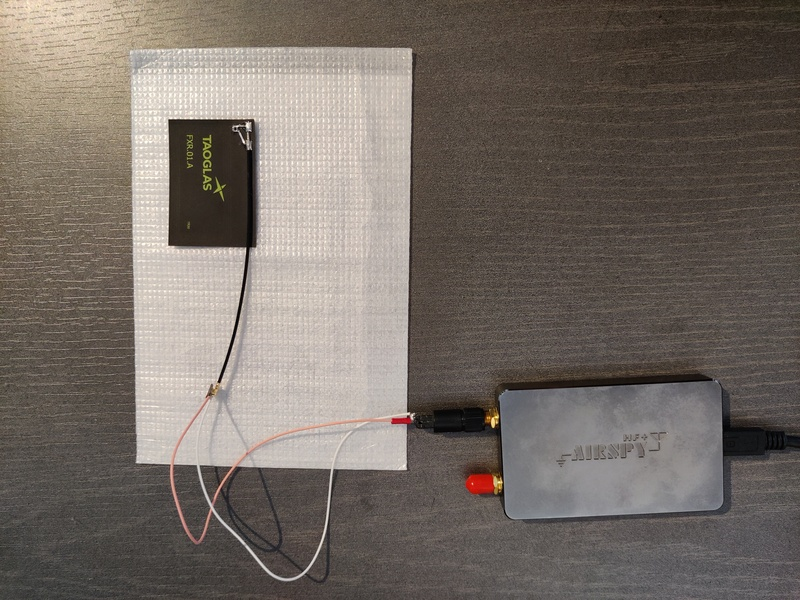
\includegraphics[scale=0.35]{figures/data_sdr-setup2.jpg}
  \caption{SDR and antenna setup}
  \label{fig:radio-setup}
\end{figure}

\subsubsection{The SDR}

LimeSDR and its shortcomings (heat, instability, freq range, sampling rate)...

Airspy HF+: made for HF, a lot more stable, noise level a lot lower, configurable...

768 kHz, 384 kHz, 192 kHz, 96 kHz and 48 kHz

\subsubsection{The "antenna"}

As described in section \ref{nfc}, NFC uses inductive coupling rather than the more common far field electromagnetic radiations. Because of this, our system needs a near-field antenna, which in this case is really just an inductor. A simple loop of copper wire qualifies as such, but in order for our antenna to be perfectly tuned to 13.56MHz, we used an industrial antenna: the Taoglas FXR.01.A\footnote{\url{https://www.taoglas.com/product/fxr01-nfc-flex-reader-antenna}}.

The antenna should be placed at least 15mm away from metallic objects, for they interfere with the magnetic field used for the communication.

As can be seen in figure \ref{fig:radio-setup}, the adapter between the SDR and the antenna is homemade using spare connectors and copper wires. The risk of interferences because of this rather unsophisticated adapter is noted, but doesn't seem to be significant later in the work.

% -------------------------------------------------------------------------------------------------------------
\subsection{Inventory of devices}

Here, we list the devices used to create the dataset. These include the PCDs (readers) and the PICCs (tags) whose communications were captured.

In terms of readers, table \ref{tab:pcd-inventory} lists the few devices used. We weren't able to find a specific NFC chip in either smartphone's characteristics. \texttt{reader2} was mostly used during the analysis phase, with the LimeSDR Mini system. The final dataset will be created with the help of \texttt{reader1}.

\begin{table}[h!]
  \centering
  \begin{tabular}{|l|l|l|}
    \hline
    \textbf{Name}    & \textbf{Type} & \textbf{Model} \\ \hline
    \textbf{reader1} & Smartphone    & OnePlus 8      \\ \hline
    \textbf{reader2} & Smartphone    & Nokia 7+       \\ \hline
  \end{tabular}
  \caption{Inventory of PCD devices}
  \label{tab:pcd-inventory}
\end{table}

On the other hand, the list of tags and their technical details can be found in table \ref{tab:picc-inventory}. A picture of tags 1 to 7 is also provided in figure \ref{fig:tags}. As the table shows, tags 1 to 5 use the exact same chip model. Tags 1 to 8 are all NFC type A compliant, while tag 9 uses the FeliCa standard from Sony. It will be interesting to contrast the classification performance between tags of the same type and between tags of different types.

On the PICCs that are marked writable, the content is harmonized to ensure the algorithm won't use the content as a feature to identify devices.

\begin{table}[h!]
  \centering
  \begin{tabular}{|l|l|l|l|l|l|l|}
    \hline
    \textbf{Name} & \textbf{NFC type} & \textbf{Standard} & \textbf{Chip}     & \textbf{Writable} & \textbf{ATQA} & \textbf{SAK} \\ \hline
    \textbf{tag1} & NFC-A             & ISO 14443-3A      & NTAG213           & Yes               & 0x0044        & 0x00         \\ \hline
    \textbf{tag2} & NFC-A             & ISO 14443-3A      & NTAG213           & Yes               & 0x0044        & 0x00         \\ \hline
    \textbf{tag3} & NFC-A             & ISO 14443-3A      & NTAG213           & Yes               & 0x0044        & 0x00         \\ \hline
    \textbf{tag4} & NFC-A             & ISO 14443-3A      & NTAG213           & Yes               & 0x0044        & 0x00         \\ \hline
    \textbf{tag5} & NFC-A             & ISO 14443-3A      & NTAG213           & Yes               & 0x0044        & 0x00         \\ \hline \hline
    \textbf{tag6} & NFC-A             & ISO 14443-3A      & Mifare Classic 1k & Yes               & 0x0004        & 0x08         \\ \hline
    \textbf{tag7} & NFC-A             & ISO 14443-3A      & Mifare Classic 1k & Yes               & 0x0004        & 0x08         \\ \hline
    \textbf{tag8} & NFC-A             & ISO 14443-4       & Mifare Classic 4k & No                & 0x0002        & 0x38         \\ \hline
    \textbf{tag9} & FeliCa            & JIS 6319-4        & RC-S967           & No                & -             & -            \\ \hline
  \end{tabular}
  \caption{Inventory of PICC devices}
  \label{tab:picc-inventory}
\end{table}

\begin{figure}[htp!]
  \centering
  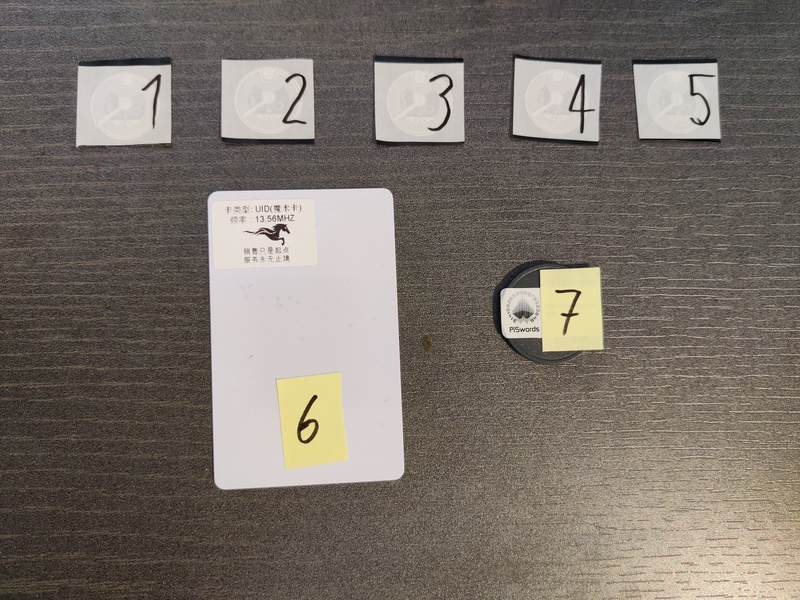
\includegraphics[scale=0.35]{figures/data_standard-tags2.jpg}
  \caption{NFC tags 1-7}
  \label{fig:tags}
\end{figure}

% -------------------------------------------------------------------------------------------------------------
\subsection{Dataset description}

\subsubsection{Requirements}

In order for the dataset to be robust, it needs to answer some basic criteria. The following list assumes the dataset will be used to train a machine learning model to discriminate between passive tags.

\begin{itemize}
  \item It should contain recordings of both very similar and very different devices.
  \item The data transmitted should not be a discriminating factor.
  \item The number of devices should be high enough to analyse scalability and generalization.
  \item Only one reader should be used to capture the data.
  \item Only one SDR should be used to capture the data.
  \item The capture's parameters should be constant across captures.
\end{itemize}

If some of those items are not met, the model trained using this data could use the content of the tags or the capture's parameters to categorize the data. It may also be unable to generalize.

\begin{figure}[htp!]
  \centering
  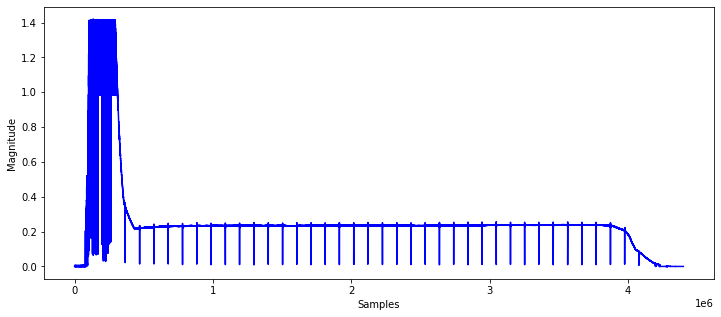
\includegraphics[scale=0.47]{figures/data_whole-transmission.png}
  \caption{\textbf{Two seconds?} of NFC communication represented as magnitudes}
  \label{fig:nfc-full}
\end{figure}

\begin{figure}[htp!]
  \centering
  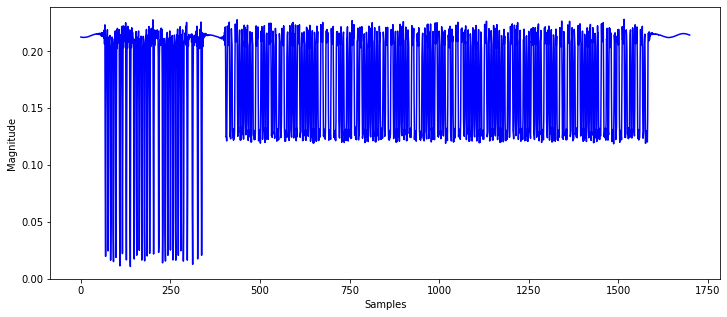
\includegraphics[scale=0.55]{figures/data_single-request-response.png}
  \caption{NFC single request/response represented as magnitudes}
  \label{fig:nfc-single}
\end{figure}

% -------------------------------------------------------------------------------------------------------------
\subsection{Validating the dataset}

\subsection{Preprocessing}
